
\chapter{Introduction}
\label{introduction}

The introductory chapter consists of the primary problem statement of the thesis,
the definition of the research questions,
a concise outline of the research methodology,
as well as
an overview of the thesis structure.

\section{Problem Statement}

% 1. Absatz: Beschreibe uns das Forschungsfeld in dem du dich befindest (DevOps / GitOps)

%\noindent
Increasingly more organizations are adopting 
a DevOps culture to develop new applications and services at high velocity. 
After all, a culture that encourages shared responsibility, transparency and rapid feedback, 
helps to narrow the gaps between teams and thus accelerate the development process.
In order to
reduce friction between engineering teams who are involved in the software development lifecycle (SDLC),
a new practice called GitOps has emerged.
It allows developers who are already familiar with the revision control system Git,
to easily deploy their applications to target environments in a self-service model.
System administrators and operators can also manage IT infrastructure
purely by interfacing with declarative state definitions stored in Git.
%GitOps is a set of principles for operating and managing software systems.
%These principles are derived from modern software operations, but also have their roots 
%in existing and widely adopted best practices. 
\bigskip

% 2. Absatz: Beschreib uns das Problem bzw. die Challenge in diesem Forschungsfeld (Was ist die Problemstellung, die es zu bearbeiten gilt)

% why is it important to solve the problem?

\noindent
GitOps as a practice for releasing software has many advantages,
but like other solutions, GitOps also has some shortcomings.
One of the unresolved problems is
the process of promoting releases between multiple deployment environments (illustrated in Figure \ref{fig:releasePromotionProcess}).

\begin{figure}[h]
	\centering
	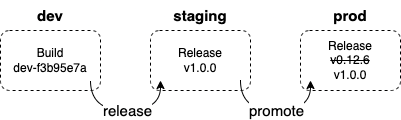
\includegraphics[width=.55\linewidth]{figures/release-promotion.drawio.png}
	\caption{release promotion process.
		%		(\citeauthor{ref}, \citeyear{ref}).
	}
	\label{fig:releasePromotionProcess}	
\end{figure}

\noindent
Current GitOps tools do not provide an integrated solution for this process,
nor do they provide any sort of abstraction for defining environments.
Users currently need to rely on separation of duties
on a file and folder level within the Git repository,
for modeling different environments.
Promotions are often achieved via hard-coded file copy operations,
which is done manually or by a
Continuous Integration (CI)/Continuous Delivery (CD) system.
Due to the nature of Git, a certain flow of promotion can not currently be enforced
(e.g. QA --> Staging --> Production).
Furthermore, for each configuration or templating tool which is used
(e.g. kustomize, helm, jsonnet, etc.),
the modeling of different deployment environments, as well as the
process of promotion, is unique.
This results in the process of promoting releases with GitOps
not being a streamlined task.
Clear guidelines and best practices,
as well as tools which implement them,
are missing in the GitOps ecosystem.
\bigskip

% 3. Absatz: Was schlägst du vor, wie man die Problemstellung bearbeiten könnte? Beschreibe uns deinen Lösugnsvorschlag dieser Arbeit, wie man das Problem bearbeiten könnte

\noindent
%
The given problem could be addressed by
providing standardised models 
for defining deployment environments and promotion processes.
%
An application programming interface (API) extension for Kubernetes
could provide custom resource definitions for these models.
%
This would allow users to define abstract representations of
their environments,
and how they want releases to be promoted between them.
%
Additional logic could be introduced into the promotion process,
like specifying a rule which ensures that new releases must first pass
certain environments or other objectives before being promoted to production.
%
The abstraction would also enable transparent replacement of the
configuration or templating tool,
while keeping the desired state definition intact.
%
Following the principles of GitOps,
an operator would ensure the continuous reconciliation
between the desired and the actual state of the resources.
\bigskip

% 4. Absatz: gib uns einen Ausblick (Paint the Big Picture) wie deine Lösung mit dem großen Ganzen zusammenhängt

\noindent
%
The proposed solution of the problem should
present a possible way of defining environments and promotion processes abstractly,
onto which future work could build upon.
%
Additionally the solution should
provide a protoype of a toolkit,
which could serve as an optional component
in addition to existing tooling within the Cloud Native Computing Foundation (CNCF).
%
Solving the problem of release promotion natively within the GitOps toolkit,
would make the adoption of GitOps more appealing,
especially for organisations, which have the need for many different environments.
%
As a result
this could generally accelerate the widespread use of GitOps
and thus enable more organisations to develop higher quality software.
%








\section{Research Questions}
\label{introduction:research-question}


% TODO: goal of this reasearch is ...
%The goal of this thesis is to
%address the problem of promoting releases between different environments in GitOps.
%\bigskip
%
%\noindent
Large organizations in particular typically have many
non-production and production environments
such as:
Development (Dev),
Quality Assurance (QA),
Staging-US,
Staging-EU,
Production-US,
Production-EU.
Usually new releases are automatically deployed to an environment,
such as QA, 
by a CI/CD system.
Now the task is to promote
new changes, which are brought about by a new release,
into subsequent or other environments.
Current GitOps tools do not have a simple answer to
the question about what is the right approach for the process of promotion.
\bigskip

%\noindent
%In particular, this thesis aims to explore
%existing strategies for the solution of the problem
%with existing tools.
%Furthermore, a prototype of a newly proposed strategy will be developed.
%Subsequently, the prototype will be tested in a laboratory experiment
%and compared to currently existing strategies.
%\bigskip

\noindent
To achieve the goal of the thesis, the following research questions (RQ) were identified:

\begin{itemize}
	\item \setword{RQ 1: How can the promotion of releases in GitOps environments be designed?}{RQ1}
	\begin{itemize}
%		\item \setword{RQ 1.1: What possibilities do existing tools offer for the promotion of releases with multiple deployment environments?}{RQ1.1}
		\item \setword{RQ 1.1: How can deployment environments, as well as promotion processes be modeled abstractly?}{RQ1.1}
		\item \setword{RQ 1.2: How can the abstract models be used to implement a standardized solution for promoting releases?}{RQ1.2}
	\end{itemize}
\end{itemize}

% ensure bullet points do not span over page break on final PDF export






\section{Research Methodology}
\label{introduction:research-methodology}

%TODO summarize chapter \ref{methodology} \nameref{methodology}

In order to help with recognition and legitimization of the conducted research,
the methodology for conducting design science (DS) research
in information systems (IS)
\autocite{designScienceResearchMethodologyForInformationSystemsResearch}
will be applied.
It consists of six activities:

\begin{itemize}
	\item \nameref{methodology:activity1}
	\item \nameref{methodology:activity2}
	\item \nameref{methodology:activity3}
	\item \nameref{methodology:activity4}
	\item \nameref{methodology:activity5}
	\item \nameref{methodology:activity6}
\end{itemize}

In activity 1,
the research problem of
release promotion with GitOps
is defined.

In activity 2,
research objectives are inferred from the problem definition in activity 1.
Each objective maps to a distinct item from the problem specification,
which helps with later evaluation in activity 5.

In activity 3,
solutions for the previously defined objectives are designed and developed
by means of producing an artifact, namely the GitOps Promotions Operator prototype.

In activity 4,
the in-context use of the artifact is demonstrated in a proof of concept.

In activity 5,
the implementation of the artifact,
and how well it supports a solution to the problem,
is evaluated.

In activity 6, as a final step,
the whole conducted research is communicated by means of
publishing it as a master thesis.

Activities 1 and 2 are supported by conducted interviews with practicing professionals in the GitOps field.
Activities 3, 4 and 5 are conducted by the researcher with the help of the prototyping method,
which means implementing the designed abstract models in a prototype, which is then demonstrated in a proof of concept and evaluated.



\section{Thesis Structure}
\label{introduction:thesis-structure}

% TODO: visualize

This thesis presents a strategy for promoting releases in GitOps environments,
and is structured as follows:

\textbf{Chapter \ref{introduction} \nameref{introduction}}:
After introducing the reader to the topic of GitOps, which can be seen as a good practice pattern within DevOps for deploying applications and generally managing systems and infrastructure as code,
the problem is briefly stated and its importance is drawn attention to.
The main goal of the thesis is outlined by stating the scientific research questions.
The research methodology, namely the used scientific methods and the general approach, is presented in a short overview.
Finally to end the introductory chapter, the structure of the thesis as a whole is described.

\textbf{Chapter \ref{related-work} \nameref{related-work}}:
%Next, the related work about this topic is discussed.
Due to the limited amount of scientific data about this topic, this chapter is quite scarce.
The suggested best practices for handling the concrete problem of release promotion with the GitOps approach,
are presented.
Furthermore the related and similar tools that are available for doing GitOps promotions are presented.
The related work chapter concludes with a summary of the chapter and draws attention to the differences
that divide the research within this thesis from other work.

\textbf{Chapter \ref{theoretical-background} \nameref{theoretical-background}}:
%The theoretical background on the topic is highlighted as a next step.
This consists of general definitions of terms that are needed for further comprehension of the thesis.
Moreover, some important concepts like DevOps, GitOps, platform engineering are described.
Latest and ongoing trends like progressive delivery, as well as
the role of Kubernetes in the current cloud native ecosystem,
are discussed.
The chapter Theoretical Background is finally rounded off with a summary,
drawing attention to what the key points are to understand,
before continuing to read the core of the thesis.

\textbf{Chapter \ref{methodology} \nameref{methodology}}:
%As the last major preparatory chapter, the research methodology is described.
First, the motivation and objectives of the chapter are outlined,
then the general approach for conducting the research of the thesis is presented,
which comprises six activities, of which the initial two are supported by conducting interviews
with practicing professionals, who have working proficiency in the GitOps field,
and the latter activities are primarily supported by the use of the prototyping method.
All used scientific methods and their concrete applications are described lastly.

\textbf{Chapter \ref{interviews} \nameref{interviews}}:
%Kicking off the empirical stages of the thesis,
%the chapter
%\ref{interviews} \nameref{interviews},
%is presented,
%in which
The research problem of promoting releases in GitOps environments is defined and motivated,
with the help of the practicing professionals from the conducted interviews.
The problem is split up into distinct problem items.
Next, for each problem item,
a solution objective is defined, which tries to provide a possible solution to a problem statement.
Each objective defines clear requirements, which have to be met by the developed artifact,
and which later help with the evaluation.

\textbf{Chapter \ref{chapter:prototype} \nameref{chapter:prototype}}:
%Representing the next and also final empirical component of the thesis,
%is the description of the developed prototype.
The asynchronous nature of GitOps deployments,
and where the developed prototype operator fits within this architecture, is brought forward.
Next, abstract models for environment and promotion resources are designed.
Then, the design of the Kubernetes custom resources for implementing the abstract models is described,
which is followed by a mockup design in YAML format of the custom resources, along with alternative mockups.
As last step in the design and development of the prototype, the custom resources are translated
to Go types, and finally
the prototype controller logic for the environment and promotion controllers is presented.
Once the design of the prototype is clear, and the implementation is developed,
the prototype is demonstrated in a proof of concept.
The demonstration is then evaluated against the solution objectives defined earlier.

\textbf{Chapter \ref{evaluation-and-results} \nameref{evaluation-and-results}}:
%The next chapter discusses the results of the conducted research,
Includes qualitative results of the interviews, as well as observed implementations
for the solution objectives and learnings from the prototyping process.
Furthermore, the research results are evaluated in a holistic manner,
by comparing the implemented solutions of the prototype to the research objectives.

\textbf{Chapter \ref{discussion-and-interpretation} \nameref{discussion-and-interpretation}}:
The thus far presented data is discussed with a holistic view,
and an interpretation by the researcher on the conducted research as a whole is given.

\textbf{Chapter \ref{future-work} \nameref{future-work}}:
Topics and ideas which were not sufficiently handled within the thesis,
as well as possible other ideas, which were brought forward by the research results or evaluation,
are presented.

\textbf{Chapter \ref{conclusion} \nameref{conclusion}}:
As a final chapter, a conclusion of the whole thesis is presented,
which includes the most important key takeaways and research results.










%Welcome to the \LaTeX{} template prepared for the Computer Science department at the university of applied sciences of Burgenland\footnote{\url{https://www.fh-burgenland.at/en/information-technology/about-the-department/}}. 
%
%Introduction, Problem, Objective, Demarcation, Question, Method, and a description of the overall structure should go into this chapter.


%
%\section{Instruction included in the original FHBgld word processor template}
%\subsection{Problem stating[!]}
%In der Problemstellung erfolgt eine Hinführung zum Thema aus dem globalen
%Zusammenhang heraus betrachtet: Warum es wichtig ist, sich mit dem konkreten
%Thema zu beschäftigen bzw. welche Bedeutung hat dieses Thema zum Beispiel für die
%Wirtschaft, Gesellschaft und Umwelt.
%\subsection{Research question and added value}
%Hier werden die konkrete(n)wissenschaftliche(n) Fragestellung(en) klar angeführt.
%Neben dem inhaltlichen Ziel der Arbeit wird fallweise auch angegeben, wie
%vorgegangen wird, um die Fragestellung zu bearbeiten (z.B. mit einem Online-
%Fragebogen). Auch die Zielgruppe der Arbeit und der für die Zielgruppe angestrebte
%Nutzen kann an dieser Stelle angeführt werden.
%Anmerkung:
%Die Erfahrung zeigt, dass es hilfreich ist, das erste Einleitungskapitel an die Betreuerin
%/ an den Betreuer zu schicken und Feedback dazu zu erhalten.
%Bitte auch darauf achten, dass alle Absatz-Abstände gleich groß sind.
%Jedes Kapitel sollte mit einem Satz beginnen und einem Satz enden und ca. mind. 1⁄2
%A4-Seite umfassen.
%
%\section{Using the \LaTeX{} template}
%
%Everything in the template revolves around the\verb|main.tex| file. Here all the other files are put together to create the thesis.
%There are three different sections to consider: 
%\begin{itemize}
%	\item Front Matter,
%	\item Chapters, and
%	\item Back Matter.
%\end{itemize}
%Each section has a folder where you can put the different parts of your thesis. In the Front Matter section you should put everything that comes before your first chapter of the thesis. Respectively, in the Back Matter section you put everything that comes after your last chapter. And finally all the chapters are put into the Chapters folder. You can put things like abstract, summaries, etc... wherever they suit your thesis. In the end it really only matters how you add them into your \verb|main.tex| file. With the \verb|\input{}| command you can add the parts if they should appear in your thesis, the order within the \verb|main.tex| also determines the order in the final pdf.
%
%\subsection{Title-page}
%The Layout of the Title-page is in the \verb|FHBgld_Thesis.cls|, normally it remains unchanged. You can use all the commands as seen in the \verb|Titlepage.tex|. 
%
%The template and also the titlepage is based on the scrbook class. So if you want to use a different class without changing the title page in the \verb|FHBgld_Thesis.cls|, it is recommended creating the title page separately and then include the compiled pdf file here, using the 
%\verb|\includepdf{<filename>}| from the \verb|pdfpages| package. Alternatively, you may use the word template for the title- page and add it using this package. In that way you can avoid any differences to the original title page template. The word templates can be found here:
%\begin{enumerate}
%	\item \url{https://moodle.fh-burgenland.at/pluginfile.php/34046/mod_folder/content/0/03_Vorlage_zur_Erstellung_wissenschaftlicher_Arbeiten\%20V2.8.docx?forcedownload=1}
%	\item \url{https://moodle.fh-burgenland.at/pluginfile.php/34046/mod_folder/content/0/03_Vorlage_zur_Erstellung_wissenschaftlicher_Arbeiten\%20V2.8\%20eng.docx?forcedownload=1}
%\end{enumerate}
%
%If you use the \verb|includepdf| package make sure that the pdf still has the correct metadata afterwards.
%
%\subsection{Citing}
%As per requirement of the FH Burgenland, the template class is configured for APA\footnote{\url{https://ctan.org/pkg/biblatex-apa?lang=en}} style: \verb|[natbib=true, backend=biber, style=apa, sorting=nty]|. It uses Biblatex and the Biber backend. The location of the bibliography file is defined in the \verb|main.tex|. Citation xamples:
%\begin{itemize}
%	\item \verb|\parencite{bibid}| provides \parencite{lamport94}
%	\item \verb|\parencite[p. 123ff]{bibid}| provides \parencite[p. 123ff]{lamport94}
%	\item \verb|\parencite{lamport94,talbot2013using}| provides \parencite{lamport94,talbot2013using}
%\end{itemize}
%
%\subsection{Temporary packages and settings}
%Some packages and settings are included to make creating your thesis easier, e.g. FixMe.
%Before building your final PDF, those should be removed. Use \verb|grep -r RMF *| in the root folder of the template to find the packages and settings that should be removed.
%
%\section{Creating the pdf}
%To create a proper pdf file of your thesis there are some things to consider
%
%\subsection{PDF build}
%The script \verb|build.sh| is provided to compile the thesis in four steps:
%\begin{enumerate}
%	\item pdflatex main.tex
%	\item biber main
%	\item bib2gls main
%	\item pdflatex main.tex
%\end{enumerate}
%\verb+bib2gls+ is used to prepare the indexes for glossaries and acronyms. Both are edited in \verb|defns.bib|, therefore, Jabref can be used to manage entries. 
%
%In case you already have your definitions in \LaTeX{} format, such as
%\begin{itemize}
%	\item \verb|\newacronym{gcd}{GCD}{Greatest Common Divisor}}|, or
%	\item \verb|\newglossaryentry{latex}{name=latex,description={Is a mark up language specially suited for scientific documents}}|
%\end{itemize}
%use \verb|convertgls2bib defns.tex defns.bib| to convert from \LaTeX{} to Bibtex.
%
%\subsection{Embed all fonts in pdf}
%Please make sure that you embed all fonts in your pdf. Also make sure all the fonts of any figures that were used in the document are embedded. 
%If you don't use any pdf figures, pdfLaTeX should embed all fonts automatically.
%
%\subsubsection{Linux}
%On Linux you can use the command \begin{verbatim}
%	pdffonts my_file.pdf
%\end{verbatim}
%to check if the fonts are embbeded. Check if all the fonts listed have a "yes" in the "emb" column. 
%\begin{verbatim}
%name                                 type              encoding         emb sub uni 
%------------------------------------ ----------------- ---------------- --- --- --- 
%BXJBCJ+NimbusSanL-Bold               Type 1            Custom           yes yes no     
%HEMYJL+NimbusSanL-Regu               Type 1            Custom           yes yes no     
%OOJWDR+SFRM1000                      Type 1            Custom           yes yes no      
%OHLNOC+SFRM0900                      Type 1            Custom           yes yes no   
%...
%\end{verbatim}
%For more information see 
%
%\url{https://www.karlrupp.net/2016/01/embed-all-fonts-in-pdfs-latex-pdflatex/}
%\subsubsection{Windows}
%On Windows using the Adobe Acrobat Reader the fonts can be found at
%\begin{verbatim}
%	File > Properties > Fonts
%\end{verbatim}
%For more information please consult
%\begin{enumerate}
%	\item \url{https://helpx.adobe.com/acrobat/using/pdf-fonts.html}
%	
%	\item \url{https://www.overleaf.com/learn/latex/Questions/My_submission_was_rejected_by_the_journal_because_%22Font_XYZ_is_not_embedded%22._What_can_I_do%3F} 
%	\end{enumerate}
%	
%	%\subsection{Making a PDF/A-1 compatible pdf}
%	\subsection{Making a PDF}
%
%	
%	\subsubsection{validation}
%	To validate the produced PDF, you can either use the Preflight tool included in Adobe Acrobat Pro or a free online version. E.g. \url{https://www.pdf-online.com/osa/validate.aspx}.
%	Please take caution as different validation tools can report different results.
%	
%	\subsubsection{metadata}
%	There may be a section in the beginning of a .tex file where you define metadata.
%	Setting your Name, Title, Subject, Keywords and remove/add Information for example. To find out what fields are possible please check here. \url{http://texdoc.net/texmf-dist/doc/latex/pdfx/pdfx.pdf#subsection.2.3}
%	
%	A file containing the metadata (jobname.xmpdata) is created when compiling. 
%	
%	Watch out, the metadata .xmpdata file is only created one time. So if you need to update it you need to clear the cache of overleaf. Or delete the .xmpdata file. It is then recreated the next time you compile. 
%	
%	\url{https://www.overleaf.com/learn/how-to/Clearing_the_cache}
%	
%	You can check the metadata of your PDF with Acrobat Reader by going to File-> properties. Or alternatively check it with an online tool.
%	
%	\subsubsection{figures}
%	As already mentioned, make sure that all the fonts used in the pictures are included. Furthermore transparency in pictures causes issues, please convert transparent figures into their nontransparent version. 
%	
%	Using Linux the command \verb|pdfimages -list <pdf>| shows the typpe of all images used. The type should always be \verb|image| and not \verb|smask|. Check and convert these images.
%	
%	\subsubsection{color}
%	Additionally, there can be problems if figures use different color spaces. Use the same command as before and check if all images use the same color. 
%	
%	If color is really important in your work it might also be a good idea to use an ICC profile for the color. 
%	For more details about colors check \url{http://texdoc.net/texmf-dist/doc/latex/pdfx/pdfx.pdf#subsection.2.5}
%	
%	It is also possible to convert the pictures automatically using ghostscript. But always check the results manually. 
%	
%	\subsubsection{Other errors}
%	Due to the complexity of Latex files there can be many more errors that are not covered here.
%	
%	The Preflight tool included in Adobe Acrobat Pro also has the ability to fix some errors. For example EOL (End of Line) errors can be fixed with its analyize and fix option. 
%	Please also check if any of the following pages might have a solution to your problem:
%	\begin{enumerate}
%		\item \url{https://www.mathstat.dal.ca/~selinger/pdfa/}
%		\item \url{https://blog.zhaw.ch/icclab/creating-pdfa-documents-for-long-term-archiving/}
%		\item german: \url{http://kulturreste.blogspot.com/2014/06/grrrr-oder-wie-man-mit-latex-vielleicht.html}
%		\item \url{https://support.stmdocs.in/wiki/?title=Generating_PDF/A_compliant_PDFs_from_pdftex}
%		\item \url{http://texdoc.net/texmf-dist/doc/latex/pdfx/pdfx.pdf}
%	\end{enumerate}
%	
%	\subsubsection{Tagged PDF}
%	Currently with Latex it is only possible to create files that are in the PDF/A-1b format. The PDF/A-1a format required the PDF to be tagged which is currently not possible in a satisfactory way.
%	A manual tagging with Adobe Acrobat Pro is possible but not recommended.
%	
%	More information about the current status of tagged pdfs can be found here:
%	\begin{enumerate}
%		\item \url{https://umij.wordpress.com/2016/08/11/the-sad-state-of-pdf-accessibility-of-latex-documents/} 
%		\item \url{https://www.tug.org/TUGboat/tb30-2/tb95moore.pdf}
%	\end{enumerate}
%	
%	\subsection{General Remarks to create the pdf}
%	Highest priority should always be the embedding of all fonts. Further compliance with the PDF/A standards is always desired, but talk to your advisor in any case.
%	
%	Please also check the following resources if you have problems and need assistance
%	
%	\begin{enumerate}
%		\item \url{https://spl29.univie.ac.at/fileadmin/user_upload/s_spl29/Studium/abschluss_master/Infoblatt_Hochschulschriften.pdf} 
%		\item \url{https://e-theses.univie.ac.at/E-Theses_erstellen_von_pdf.pdf}
%	\end{enumerate}
%	
%	\section{Further tips on the template}
%	In the following chapters there are some general tips on the elements of Latex. You can check them out if you think they have useful information for you. Then you delete these chapters and replace them with the real chapters of your thesis.
